\documentclass{article}
\usepackage[final,main]{neurips_2025}  % NEURIPS style (neurips_2025.sty is in paper_draft/)

\usepackage[utf8]{inputenc}
\usepackage[T1]{fontenc}
\usepackage[hidelinks]{hyperref}  % REQUIRED: clickable links
\usepackage{url}
\usepackage{booktabs}  % REQUIRED: professional tables
\usepackage{graphicx}
\usepackage{amsmath,amssymb}
\usepackage{subcaption}
\usepackage{enumitem}
\usepackage{natbib}
\usepackage{algorithm}
\usepackage[noend]{algpseudocode}

% Import command files
\input{commands/math}
\input{commands/general}
\input{commands/macros}

% Use this bibliography style:
\bibliographystyle{plainnat}

\title{When Does Neural-Symbolic Integration \emph{Understand}?\\
Data Efficiency, Reasoning Shortcuts, and Compositional\\
Generalization on MNIST-Addition}

\author{Chenhao Tan and NeuriCo}

\begin{document}
\maketitle

\begin{abstract}
Neuro-symbolic (NeSy) systems promise to combine neural perception with symbolic reasoning,
yielding data efficiency, interpretable symbols, and compositional reuse. But these promises rest
on a hidden assumption: that the system actually \emph{grounds} its latent symbols correctly. We
ask, on the canonical \mnistadd benchmark, when wiring a fixed symbolic ``$+$'' into a shared neural
digit classifier---trained only on the \emph{sum} of two images, never on the digits themselves---
produces genuine perception-plus-reasoning, and when it only appears to. Across 210 training runs
(5 seeds per configuration), we report four findings measured side by side with confidence intervals
and significance tests. First, integration is a large data-efficiency win: at 1{,}000 training pairs
the NeSy model reaches $85.4\%$ sum accuracy versus $22.0\%$ for a pure-neural baseline (Welch
$p{=}2.9{\times}10^{-13}$), matching a fully digit-supervised oracle. Second, high task accuracy can
hide a broken model: changing only the symbolic operator to $(a{+}b)\bmod 10$ makes correct grounding
\emph{never} emerge---raw grounding $\approx0.1\%$ among seeds that learn the task---because the
network reads digits via a systematic relabeling that leaves the modular sum invariant, a reasoning
shortcut visible only when grounding is measured permutation-aligned. Third, just $10$ labeled images
(one per class) eliminate the shortcut and stabilize training (grounding $\approx0.1\%\to97.7\%$),
whereas unsupervised regularizers do not. Fourth, correct grounding unlocks zero-shot compositional
generalization to $2$- and $3$-digit addition ($95.7\%$/$93.7\%$) that the neural baseline structurally
cannot achieve ($0\%$). The lesson for practitioners: task accuracy is not enough; grounding must be
measured, the operator's symmetry determines whether symbols are identifiable, and a pinch of symbol
supervision is a cheap, decisive fix.

\end{abstract}

\section{Introduction}
\label{sec:intro}

Neuro-symbolic (NeSy) AI sets out to build a single system that \emph{perceives} with neural networks
and \emph{reasons} with symbolic structure~\citep{garcez2020,marra2021}. The appeal is concrete: by
factoring a task into ``recognize the parts'' and ``combine them with known rules,'' a NeSy model
should learn from far less data, expose interpretable intermediate symbols, and reuse those symbols
to solve problems it was never trained on. The canonical demonstration is \mnistadd
\citep{manhaeve2018}: a model sees two digit images and is supervised only on their \emph{sum}, never
on the digits, yet is expected to learn to read digits as a by-product of learning to add.

\para{The promise hides an assumption.} Every downstream NeSy benefit---interpretability, knowledge
reuse, compositional generalization---depends on the latent symbols being \emph{correct}. If the
network learns a mapping from images to symbols that is systematically wrong but still produces the
right final answer, the system has not understood anything; it has found a \newterm{reasoning
shortcut}~\citep{li2024softened,deepsymbolic2022}. A practitioner who watches only task accuracy
will never notice. This is not a hypothetical: with only distant supervision, the perception-to-symbol
map is under-constrained, and training can collapse onto a spurious but self-consistent solution.

\para{What is missing.} The two headline NeSy claims---data efficiency and correct
grounding---are widely asserted but rarely measured together with statistical rigor on identical
splits. Data efficiency is seldom reported head-to-head against a neural baseline with confidence
intervals, and \emph{grounding accuracy is almost never reported at all}, so reasoning shortcuts stay
invisible. Prior work raises the shortcut problem qualitatively, but a controlled, multi-seed
\emph{measurement} of \emph{when} shortcuts appear, \emph{what they look like}, and \emph{which cheap
fixes work} has been missing.

\para{Our approach.} We run a single controlled study on \mnistadd that measures four quantities
side by side, on identical splits, across $5$ seeds, with Welch $t$-tests, Holm--Bonferroni
correction, and Cohen's $d$ effect sizes. We compare three models on a \emph{shared} CNN encoder so
the only variable is the learning signal: a \neural baseline that predicts the sum directly, a
\nesy model that outputs per-image digit distributions and computes the sum by exact differentiable
marginalization (the DeepProbLog/Scallop idea in compact form), and an \oracle trained on true digit
labels as an upper bound. The study is held together by one clean manipulation: \emph{flipping a single
symbolic operator}, standard addition $a{+}b$ versus modular addition \modten, which turns reasoning
shortcuts on and off while everything else---architecture, data, optimizer---stays fixed.

\para{What we find.} (i) Integration is a large, statistically significant data-efficiency win:
at $1{,}000$ pairs the \nesy model reaches $85.4\%$ sum accuracy versus the neural baseline's
$22.0\%$ (Cohen's $d{=}56$, $p{=}2.9{\times}10^{-13}$), recovering digits at $92$--$99\%$ with no
digit labels. (ii) Yet under the modular operator, correct grounding \emph{never} emerges: among
seeds that learn the task, raw grounding is $\approx0.1\%$, while a permutation-aligned metric reveals
a clean systematic relabeling---sometimes the exact cyclic shift $d\mapsto(d{+}5)\bmod 10$. The
oracle grounds at $99\%$ on the \emph{same} task, so the failure is caused by distant supervision under
a symmetric operator, not by the task being hard. (iii) Just $10$ labeled images break the symmetry
and restore grounding to $97.7\%$ in every seed; unsupervised regularizers do not. (iv) With correct
grounding, the \nesy model solves $2$- and $3$-digit addition it never saw at $95.7\%$/$93.7\%$ by
composing its digit classifier with a symbolic place-value sum, while the neural baseline scores
exactly $0\%$.

\para{Contributions.}
\begin{itemize}[leftmargin=*,itemsep=0pt,topsep=0pt]
    \item We quantify NeSy data efficiency head-to-head against a neural baseline and a digit-supervised
    oracle on identical splits, with confidence intervals and effect sizes at six training sizes.
    \item We introduce a permutation-aware (Hungarian-aligned) grounding diagnostic and use a
    single-operator flip ($a{+}b$ vs.\ \modten) to show that whether high task accuracy implies correct
    symbols is a property of the \emph{task's symmetry}, not of NeSy in general.
    \item We compare cheap mitigations and show that a handful of labeled symbols ($10$ images) is the
    decisive, reliable fix for a detected shortcut, while unsupervised priors are not.
    \item We demonstrate that correct grounding unlocks zero-shot compositional generalization to
    multi-digit addition---a capability the neural baseline structurally lacks.
\end{itemize}

The rest of the paper reviews related work (\secref{sec:related}), details our models, operators, and
metrics (\secref{sec:method}), presents results E1--E5 (\secref{sec:results}), discusses
interpretation and limitations (\secref{sec:discussion}), and concludes (\secref{sec:conclusion}).

\section{Related Work}
\label{sec:related}

\para{Probabilistic logic with neural predicates.} A major NeSy family compiles logic into a
differentiable circuit and lets a neural network supply the probabilities of atoms. DeepProbLog
\citep{manhaeve2018} adds a neural predicate to ProbLog, compiles inference to arithmetic circuits, and
introduces \mnistadd as its flagship benchmark; NeurASP \citep{yang2020} couples network softmax
outputs to an answer-set program; and Scallop \citep{li2023scallop} implements differentiable Datalog
with provenance semirings and a tunable top-$k$ approximation for scale. Our \nesy model is a compact
re-implementation of the shared core of these systems: per-image digit distributions combined by an
\emph{exact} differentiable marginalization over digit pairs. We do not benchmark the toolkits
themselves; we use their common mechanism as a clean experimental substrate and add the grounding and
shortcut measurements they usually omit.

\para{Differentiable logic as loss or representation.} A second family treats knowledge as a soft
constraint on network outputs rather than as architecture. Logic Tensor Networks \citep{badreddine2020}
define a many-valued differentiable first-order logic whose formulas become satisfiability objectives,
and the semantic loss \citep{xu2017} measures the distance of network outputs from satisfying a logical
constraint. These methods inject knowledge without changing the architecture; we instead bake the
symbolic operator directly into the forward computation, which is precisely what makes the latent
digit symbols inspectable and the grounding question well posed.

\para{The symbol grounding problem and reasoning shortcuts.} The closest work to ours studies how
distant supervision under-constrains the perception-to-symbol map. Softened Symbol Grounding
\citep{li2024softened} and Deep Symbolic Learning \citep{deepsymbolic2022} observe that a NeSy system
can reach high task accuracy while learning a wrong, self-consistent symbol map, and propose training
schemes to mitigate it. These works raise the shortcut problem largely qualitatively. We complement
them with a controlled, multi-seed \emph{measurement}: we tie shortcut emergence to a concrete,
analyzable property of the symbolic operator (its symmetry), provide a permutation-aware detector,
quantify the resulting collapse and its training instability, and rank cheap mitigations against one
another.

\para{Compositional and out-of-distribution generalization.} Modular neuro-symbolic systems such as
NS-VQA \citep{yi2018} and the Neuro-Symbolic Concept Learner \citep{mao2019} achieve strong
compositional generalization by pairing a neural perception front-end with a symbolic executor, and
multi-digit/multi-addend addition is a standard stress test for inference scaling
\citep{manhaeve2018,li2023scallop}. We use multi-digit addition differently: as a \emph{diagnostic of
grounding}. Because our single-digit classifier can be composed with a symbolic place-value sum, a
model with correct grounding should generalize zero-shot while one with a shortcut should not, making
OOD accuracy a direct, externally checkable test of whether the latent symbols are right.

\para{Surveys and positioning.} Broad treatments of the field
\citep{garcez2020,marra2021} catalog the design space and repeatedly flag two gaps: data efficiency is
asserted more than measured, and grounding is under-reported. Our study is deliberately narrow---one
benchmark, one perceptual domain---but addresses exactly these gaps with statistics, and ties data
efficiency, grounding, mitigation, and compositional generalization together through a single operator
manipulation.

\section{Methodology}
\label{sec:method}

\subsection{Problem setup}
\mnistadd presents pairs of digit images $(\vx_1,\vx_2)$ with only the integer sum
$s = y_1 + y_2$ supervised; the true digit labels $(y_1,y_2)$ are hidden during training. The learning
challenge is that the digit-recognition map must be discovered purely as a by-product of fitting the
sum---this is what makes the benchmark a clean test of perception-via-symbolic-constraint, and what
makes correct \emph{grounding} a non-trivial outcome.

\subsection{Models}
All three models share an identical LeNet-style CNN encoder; the \emph{only} difference is the output
head and the learning signal, which isolates the symbolic structure as the variable.

\para{Neural-only baseline.} The shared encoder is applied to each image; the two feature vectors are
concatenated and passed to an MLP that produces a $19$-way softmax over possible sums $\{0,\dots,18\}$
(a $10$-way head for the modular task). It has no knowledge that the output decomposes as $d_1{+}d_2$.

\para{Neuro-symbolic (\nesy).} The shared encoder maps each image to a $10$-way digit
log-probability vector. Treating the two digits as independent given the images, the distribution over
the sum is computed \emph{exactly and differentiably} as the convolution of the two digit pmfs,
\begin{equation}
\label{eq:marginalization}
P(\text{sum}=s) \;=\; \sum_{a+b=s} P(d_1{=}a)\,P(d_2{=}b),
\end{equation}
which is the DeepProbLog/Scallop marginalization in compact form. Training minimizes the negative
log-likelihood of the \emph{true sum only} (distant supervision). The symbolic operator is fixed and
never learned. For the modular task, the constraint in \eqref{eq:marginalization} becomes
$a{+}b\equiv s \pmod{10}$.

\para{Oracle (upper bound).} The same $10$-way CNN is trained with ordinary cross-entropy on the true
digit labels and adds via argmax. It bounds the achievable grounding and sum accuracy and, crucially,
serves as a control: because it sees digit labels, it should ground correctly \emph{regardless} of the
symbolic operator.

\subsection{Symbolic operators: a controlled shortcut switch}
We study two operators that differ only in their algebra.
\emph{Standard addition} ($a{+}b$, output $0$--$18$) has boundary constraints---a sum of $0$ forces
$0{+}0$ and a sum of $18$ forces $9{+}9$---that uniquely pin the symbols, making the grounding
identifiable. \emph{Modular addition} \modten (output $0$--$9$) deliberately removes those boundary
constraints and introduces a rotational symmetry: any cyclic relabeling $d\mapsto(d{+}k)\bmod 10$
applied to both images leaves the modular sum invariant. The operator therefore \emph{admits} an exact
affine shortcut and is expected to \emph{induce} one under distant supervision. The oracle is unaffected
because it never relies on the sum to identify digits. This single-operator flip is the backbone of our
study: it switches shortcuts on and off while holding architecture, data, and optimization fixed.

\subsection{Data}
We use the locally pre-built \mnistadd dataset ($30{,}000$ train pairs, $5{,}000$ test pairs) indexing
into MNIST. True digit labels are used \emph{only} for evaluation (grounding) and for the oracle and
mitigation conditions. We verified data integrity (stored sums equal the sums of the true digits; test
indices map exactly to the MNIST test images). For the compositional experiment we deterministically
synthesize $2$- and $3$-digit number-addition test sets ($5{,}000$ examples each) from MNIST test
images.

\subsection{Metrics}
\begin{itemize}[leftmargin=*,itemsep=0pt,topsep=0pt]
    \item \para{Test sum accuracy} --- the primary task metric.
    \item \para{Digit-grounding accuracy} --- \emph{raw} (argmax digit vs.\ true label) and
    \emph{Hungarian-aligned} (accuracy under the best $10{\times}10$ label permutation, found by solving
    the assignment problem). When aligned grounding greatly exceeds raw grounding, the network has
    learned a \emph{systematic} relabeling---a reasoning shortcut. We flag a shortcut when
    aligned${-}$raw${>}0.10$.
    \item \para{Compositional OOD accuracy} --- multi-digit addition solved by a single-digit-trained
    model via symbolic place-value composition.
    \item \para{Training wall-clock} --- secondary.
\end{itemize}

\subsection{Protocol and reproducibility}
We run $5$ seeds $\{0,\dots,4\}$ per configuration and report mean ${\pm}\,95\%$ $t$-based confidence
intervals. The primary test is Welch's two-sample $t$-test (unequal variance) for \nesy vs.\ \neural at
each training size, with Holm--Bonferroni correction across the six sizes and Cohen's $d$ effect sizes;
for the compositional analysis we report Pearson correlation. All conditions use the same
hyperparameters (12 epochs, batch size 128, Adam at $10^{-3}$), set in \texttt{src/config.py}; seeds are
fixed for Python/NumPy/PyTorch. The full grid (E1+E5 $=165$ runs, E3 $=30$, E4 $=15$) runs in roughly
five minutes across three GPUs on an NVIDIA RTX A6000 (PyTorch 2.12, CUDA). Raw per-run results, the
aggregate statistics, and figures are saved under \texttt{results/} and \texttt{figures/}.

\section{Results}
\label{sec:results}

We organize results around the four hypotheses: data efficiency (E1), grounding and its silent failure
under a flipped operator (E2/E5), mitigations (E3/E5), and compositional generalization (E4).

\subsection{E1 --- Data efficiency: integration is a large, significant win at every size}
\label{sec:e1}

\Tabref{tab:e1} and \figref{fig:data_efficiency}(a) compare the three models across six training
sizes on standard addition. The \nesy model beats the \neural baseline at \emph{every} size (all
Holm-adjusted $p{<}0.01$), tracks the oracle closely, and the gap is largest in the low-data regime.
The single most striking point is at $1{,}000$ pairs, where \nesy reaches $85.4\%$ versus the
baseline's $22.0\%$---a Cohen's $d$ of $56$ ($p{=}2.9{\times}10^{-13}$). The neural baseline needs
roughly $5{,}000$ pairs to reach what \nesy achieves with about $1{,}000$. As data grows the gap
shrinks but never closes (e.g.\ $+1.0$ point at $30{,}000$, still $p{<}0.01$), exactly the pattern the
data-efficiency claim predicts.

\begin{table}[t]
    \centering
    \resizebox{\textwidth}{!}{%
    \begin{tabular}{@{}rccccccc@{}}
        \toprule
        \textbf{\# train pairs} & \textbf{\neural} & \textbf{\nesy (sum-only)} & \textbf{\oracle}
        & \textbf{\nesy$-$\neural} & \textbf{Cohen's $d$} & \textbf{Welch $p$ (raw)}
        & \textbf{Holm-adj.\ $p$} \\
        \midrule
        100    & 0.086 & \textbf{0.130} & 0.429 & $+0.044$ & 2.28  & $8.8{\times}10^{-3}$  & $8.8{\times}10^{-3}$ \\
        500    & 0.130 & \textbf{0.649} & 0.794 & $+0.519$ & 5.43  & $9.3{\times}10^{-4}$  & $1.9{\times}10^{-3}$ \\
        1{,}000  & 0.220 & \textbf{0.854} & 0.868 & $+0.634$ & 56.3  & $2.9{\times}10^{-13}$ & $1.7{\times}10^{-12}$ \\
        5{,}000  & 0.883 & \textbf{0.955} & 0.958 & $+0.072$ & 10.25 & $1.6{\times}10^{-6}$  & $7.9{\times}10^{-6}$ \\
        15{,}000 & 0.952 & \textbf{0.973} & 0.975 & $+0.021$ & 4.82  & $3.8{\times}10^{-4}$  & $1.5{\times}10^{-3}$ \\
        30{,}000 & 0.970 & \textbf{0.980} & 0.981 & $+0.010$ & 4.13  & $4.8{\times}10^{-4}$  & $1.5{\times}10^{-3}$ \\
        \bottomrule
    \end{tabular}
    }
    \caption{\textbf{E1: data efficiency on standard addition.} Test sum accuracy (mean over $5$ seeds);
    \nesy is the sum-only neuro-symbolic model, \oracle is digit-supervised. \nesy beats the \neural
    baseline at every training size, with the largest gap at $1{,}000$ pairs ($d{=}56.3$). Every
    Holm-adjusted $p{<}0.01$, so all comparisons remain significant after family-wise correction. Best
    of \{\neural, \nesy\} in \textbf{bold}.}
    \label{tab:e1}
\end{table}


\subsection{E2 --- Grounding emerges without any digit labels (standard addition)}
\label{sec:e2}

\figref{fig:data_efficiency}(b) shows that \nesy's latent digit-grounding rises from $28.3\%$
(100 pairs) to $99.0\%$ ($30$k pairs), essentially matching the digit-supervised oracle---even though
\nesy never saw a digit label. The Hungarian-aligned grounding \emph{equals} the raw grounding at every
size ($0/5$ shortcut flags throughout), so standard \mnistadd is \newterm{shortcut-robust}: its boundary
sums uniquely pin the symbols. The visible sum-vs-grounding gap (e.g.\ $85.4\%$ sum vs.\ $92.4\%$
grounding at $1$k) is just the ``both digits must be right'' effect (sum~$\approx$~grounding$^2$), not a
shortcut.

\begin{figure}[t]
    \centering
    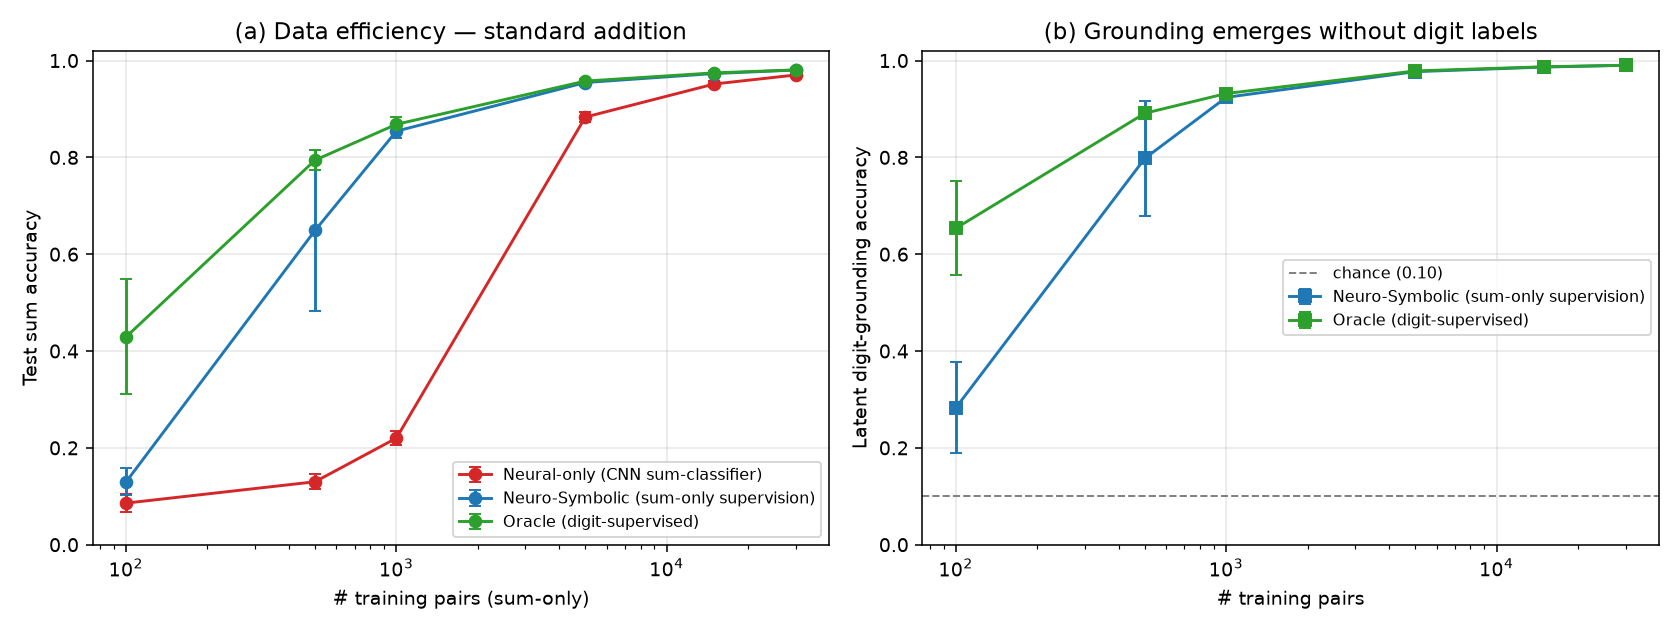
\includegraphics[width=0.95\linewidth]{figures/fig1_data_efficiency.png}
    \caption{\figleft Data efficiency on standard addition. \nesy (blue) dramatically beats the
    \neural baseline (red), most sharply in the low-data regime, and tracks the digit-supervised oracle
    (green); the baseline needs ${\sim}5{\times}$ more data to catch up. \figright Latent
    digit-grounding accuracy rises to $99\%$ for \nesy with \emph{no} digit labels, matching the oracle
    and far above the $0.10$ chance line. Error bars are $95\%$ confidence intervals over $5$ seeds.}
    \label{fig:data_efficiency}
\end{figure}

\subsection{E5 --- Flip the operator and grounding collapses}
\label{sec:e5}

Changing \emph{only} the symbolic operator to \modten produces a sharp dissociation between task
accuracy and grounding (\Tabref{tab:e5}, \twofigref{fig:shortcut}{fig:confusion}). Standard addition
grounds at $99.0\%$; modular addition grounds at $\approx2\%$ raw. Among the four seeds that actually
learn the modular task (sum${>}0.3$), raw grounding is just $0.09\%$ (max $0.16\%$): the network reads
the digits systematically wrong via a global relabeling that leaves \modten invariant. The
permutation-aligned metric makes the failure legible---aligned grounding is $0.53$--$0.60$ on shortcut
seeds and reaches $0.99$ on the cleanest realization, where the model lands on the \emph{exact}
predicted cyclic shift $d\mapsto(d{+}5)\bmod 10$ (\figref{fig:confusion}). The fifth seed collapses to
predicting a single class. Crucially, the digit-supervised \emph{oracle grounds at $99.0\%$ on the
identical modular task}, so the collapse is caused by distant supervision under a symmetric operator,
not by the task. The standard-vs-modular grounding contrast is overwhelming ($0.990$ vs.\ $0.020$,
Welch $p{=}9.6{\times}10^{-7}$, $d{=}31.5$). This shortcut is visible \emph{only} because we measured
grounding; task accuracy alone is blind to it.

\begin{table}[t]
    \centering
    \resizebox{\textwidth}{!}{%
    \begin{tabular}{@{}lcccl@{}}
        \toprule
        \textbf{Task (\nesy, $N{=}30$k)} & \textbf{Sum acc (mean${\pm}$CI)} & \textbf{Grounding (raw)}
        & \textbf{Hungarian-aligned} & \textbf{Outcome over $5$ seeds} \\
        \midrule
        standard $a{+}b$ & $0.980 \pm 0.002$ & \textbf{0.990} & 0.990 & $0/5$ shortcut (grounds correctly) \\
        modular \modten & $0.657 \pm 0.380$ & \textbf{0.020} & 0.471 & \textbf{$4/5$ shortcut $+$ $1/5$ collapse} \\
        modular --- \oracle (digit-sup.) & 0.979 & \textbf{0.990} & 0.990 & $0/5$ (control: same task, grounds fine) \\
        \bottomrule
    \end{tabular}
    }
    \caption{\textbf{E5: flipping the operator switches shortcuts on.} Changing only $a{+}b\to\modten$
    leaves task accuracy non-trivial but collapses raw grounding from $0.990$ to $0.020$; the large
    aligned${-}$raw gap reveals a systematic relabeling. The digit-supervised oracle grounds at $0.990$
    on the \emph{same} modular task (control), so the failure is caused by distant supervision under a
    symmetric operator. Standard vs.\ modular grounding: Welch $p{=}9.6{\times}10^{-7}$, $d{=}31.5$.}
    \label{tab:e5}
\end{table}


\begin{figure}[t]
    \centering
    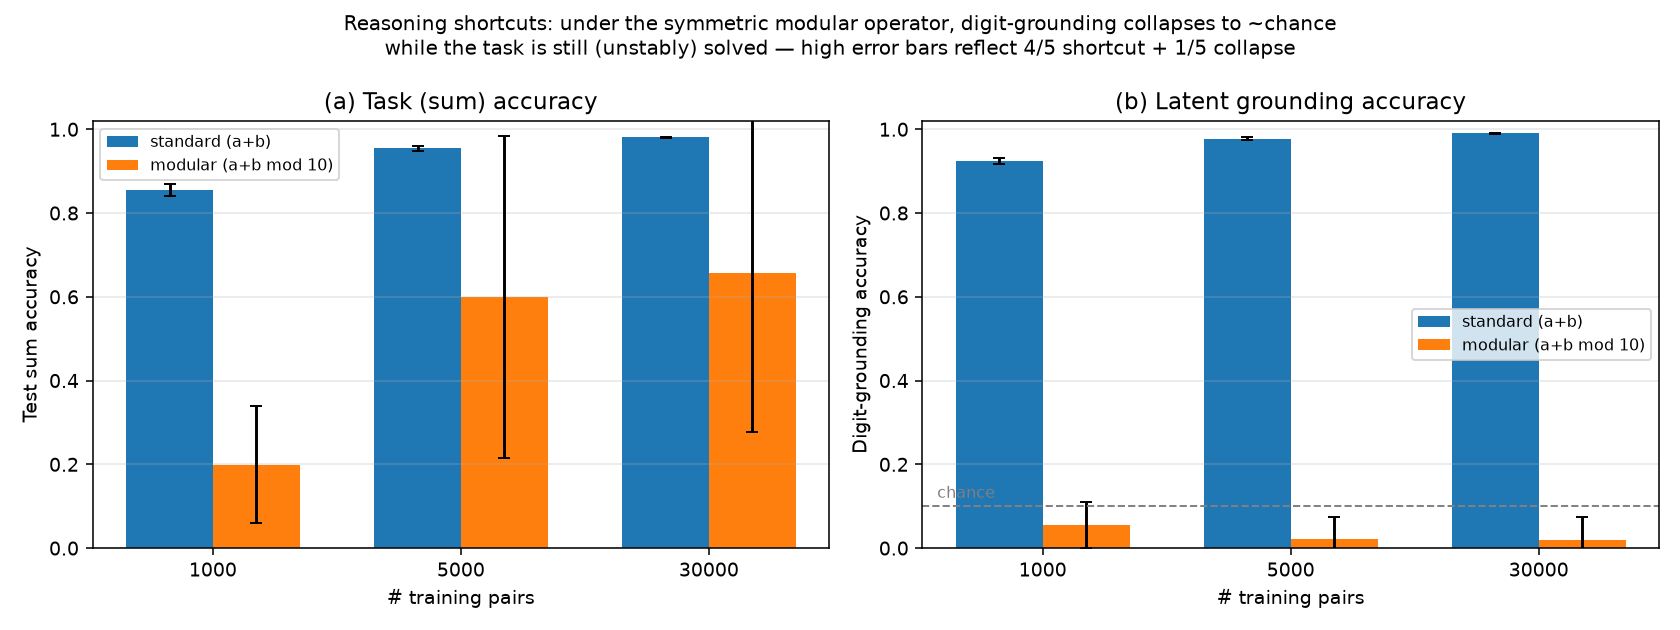
\includegraphics[width=0.95\linewidth]{figures/fig2_shortcut.png}
    \caption{Flipping one operator switches reasoning shortcuts on. \figleft Task (sum) accuracy:
    standard addition (blue) is high and stable, while modular addition (orange) is solved
    \emph{unstably}---the large error bars reflect $4/5$ seeds finding a shortcut and $1/5$ collapsing.
    \figright Latent grounding: standard addition reaches $99\%$, but modular addition sits near the
    $0.10$ chance line---high task accuracy with near-zero grounding. Bars are means over $5$ seeds;
    error bars are $95\%$ confidence intervals.}
    \label{fig:shortcut}
\end{figure}

\begin{figure}[t]
    \centering
    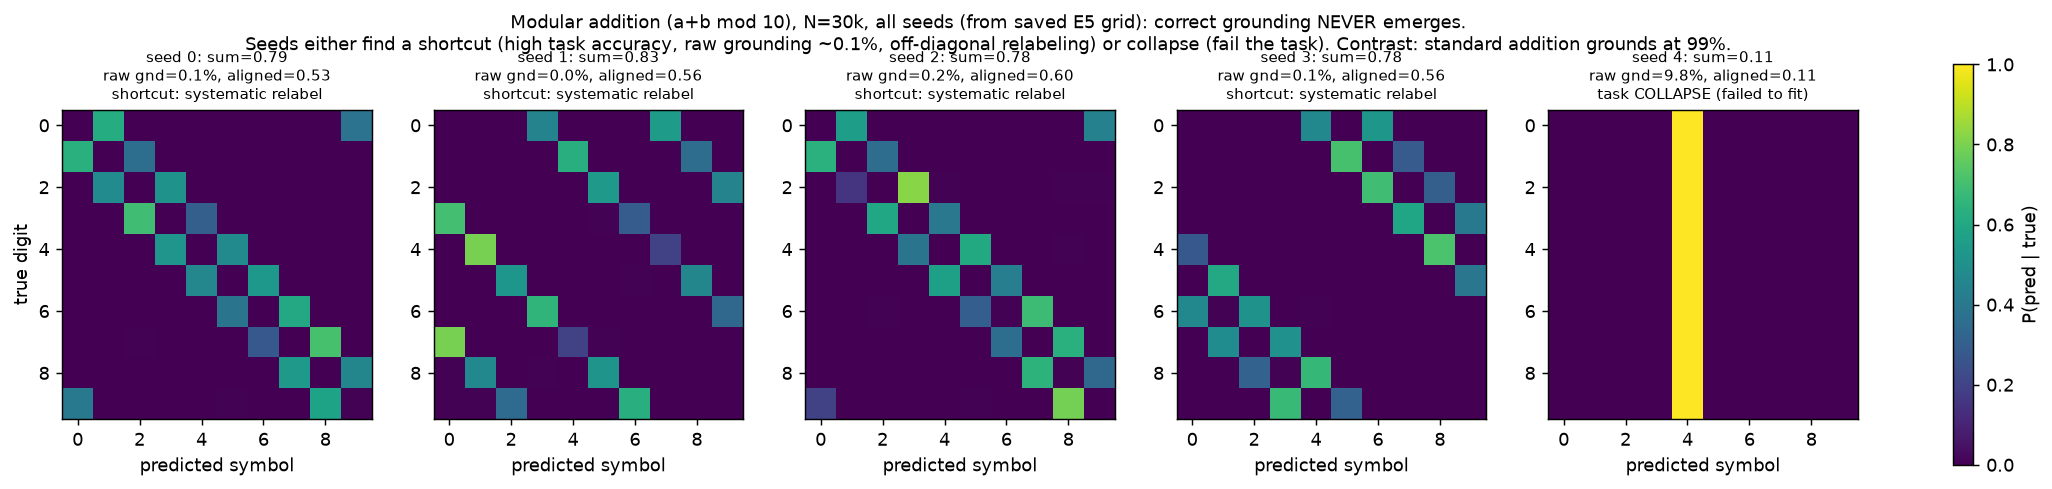
\includegraphics[width=0.98\linewidth]{figures/fig3_confusion.png}
    \caption{Per-seed grounding confusion matrices (rows: true digit, columns: predicted symbol) for
    modular addition at $N{=}30$k, read from the saved E5 grid. Seeds 0--3 place nearly all mass
    \emph{off} the diagonal: a clean, systematic relabeling (a reasoning shortcut) rather than random
    noise---seed 1 is close to the exact $d\mapsto(d{+}5)$ cyclic shift. Seed 4 collapses to a single
    predicted class (failed to fit). Correct grounding never appears, whereas standard addition grounds
    on the diagonal at $99\%$.}
    \label{fig:confusion}
\end{figure}

\subsection{E3/E5 --- Mitigations: needed and effective exactly when a shortcut exists}
\label{sec:e3}

\Tabref{tab:e3} and \figref{fig:mitigations} report grounding accuracy under each intervention. We
evaluate standard addition at $N{=}1$k (where its grounding gap is largest) and modular addition at
$N{=}5$k (where the shortcut is firmly established); each column is a within-task before/after
comparison, so the differing $N$ does not affect the conclusion. On standard addition, where there is no
shortcut to fix, mitigations do essentially nothing. On modular addition, \emph{just $10$ labeled
images} (one per class) break the symmetry and restore grounding from $\approx0.1\%$ to $97.7\%$ in
\emph{every} seed (per-seed $0.973$--$0.981$; Welch $p{=}1.6{\times}10^{-3}$, $d{=}4.8$), while also
stabilizing training (sum accuracy $\to0.954$, no collapses). Adding more labels ($50$, $200$) does not
help further. Unsupervised regularizers are unreliable: a marginal-uniformity prior recovers only
partial grounding ($0.390$, high variance) and an entropy penalty does not help at all ($0.128$). The
cure matches the disease---supply the missing identifying constraint---and it is extremely cheap.

\begin{table}[t]
    \centering
    \begin{tabular}{@{}lcc@{}}
        \toprule
        \textbf{Intervention} & \textbf{Standard add @$N{=}1$k} & \textbf{Modular add @$N{=}5$k} \\
         & \textbf{(no shortcut)} & \textbf{(shortcut present)} \\
        \midrule
        baseline (none)                              & 0.924 & 0.116 \footnotesize{(4/5 $\approx$0; 1 seed 0.57)} \\
        $+$ aux digit labels, 1/class (10 total)     & 0.925 & \textbf{0.977} \\
        $+$ aux 5/class (50 total)                   & 0.926 & 0.977 \\
        $+$ aux 20/class (200 total)                 & 0.931 & 0.979 \\
        $+$ marginal-uniformity prior                & 0.924 & 0.390 \\
        $+$ entropy regularization                   & 0.925 & 0.128 \\
        \bottomrule
    \end{tabular}
    \caption{\textbf{E3: mitigations restore grounding only when a shortcut exists.} Digit-grounding
    accuracy under each intervention (standard addition evaluated at $N{=}1$k, modular at $N{=}5$k; each
    column is a within-task before/after). On standard addition there is nothing to fix. On modular
    addition, just $10$ labeled images break the symmetry and restore grounding to $0.977$ in every seed
    (Welch $p{=}1.6{\times}10^{-3}$, $d{=}4.8$), whereas unsupervised regularizers help only partially
    (uniform prior) or not at all (entropy). Best modular result in \textbf{bold}.}
    \label{tab:e3}
\end{table}


\begin{figure}[t]
    \centering
    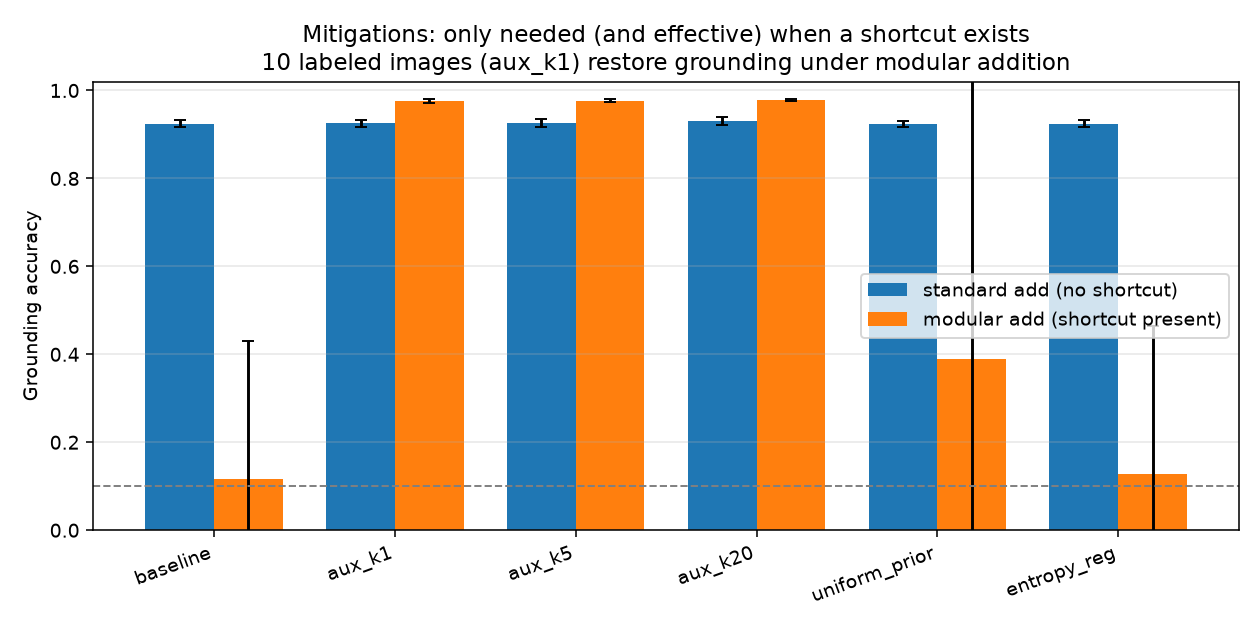
\includegraphics[width=0.85\linewidth]{figures/fig5_mitigations.png}
    \caption{Mitigations are needed (and effective) only when a shortcut exists. On standard addition
    (blue, no shortcut) all interventions leave grounding essentially unchanged. On modular addition
    (orange, shortcut present) just $10$ labeled images (\texttt{aux\_k1}) restore grounding to
    $97.7\%$; more labels add nothing, the uniform prior helps only partially (high variance), and the
    entropy penalty does not help. Dashed line is the $0.10$ chance level.}
    \label{fig:mitigations}
\end{figure}

\subsection{E4 --- Compositional generalization: the payoff of correct grounding}
\label{sec:e4}

Finally, \Tabref{tab:e4} and \figref{fig:ood} show the capability that correct grounding unlocks.
Trained on \emph{single-digit} sums only, the \nesy model solves $2$- and $3$-digit number addition it
never saw---at $95.7\%$ and $93.7\%$---by composing its digit classifier with a symbolic place-value
sum, essentially matching the oracle ($96.0\%$/$94.0\%$). The \neural baseline scores exactly $0\%$: it
cannot even emit sums in this range, a structural rather than a tuning failure. Across the grounded
models, single-digit grounding and OOD accuracy correlate almost perfectly (Pearson $r{=}0.993$,
$p{=}1{\times}10^{-8}$), but because that correlation spans models that all ground well, we treat the
\emph{categorical} contrast ($0\%$ for the ungrounded baseline vs.\ ${\sim}96\%$ for grounded models) as
the stronger evidence. This is the most direct demonstration that integration buys a genuinely new
capability, not just a higher benchmark number---and that the capability rests on correct grounding.

\begin{table}[t]
    \centering
    \begin{tabular}{@{}lccc@{}}
        \toprule
        \textbf{Model} & \textbf{2-digit (OOD)} & \textbf{3-digit (OOD)} & \textbf{single-digit grounding} \\
        \midrule
        \neural          & 0.000 & 0.000 & 0.000 (n/a) \\
        \nesy            & \textbf{0.957} & \textbf{0.937} & 0.990 \\
        \oracle          & 0.960 & 0.940 & 0.990 \\
        \bottomrule
    \end{tabular}
    \caption{\textbf{E4: compositional generalization.} Models trained only on single-digit sums,
    evaluated zero-shot on multi-digit number addition via symbolic place-value composition. \nesy nearly
    matches the oracle and generalizes to a structure it never saw, \emph{because} its grounding is
    correct; the \neural baseline cannot represent outputs in this range (structural $0\%$). Best of the
    two learnable contrasts (\neural, \nesy) in \textbf{bold}.}
    \label{tab:e4}
\end{table}


\begin{figure}[t]
    \centering
    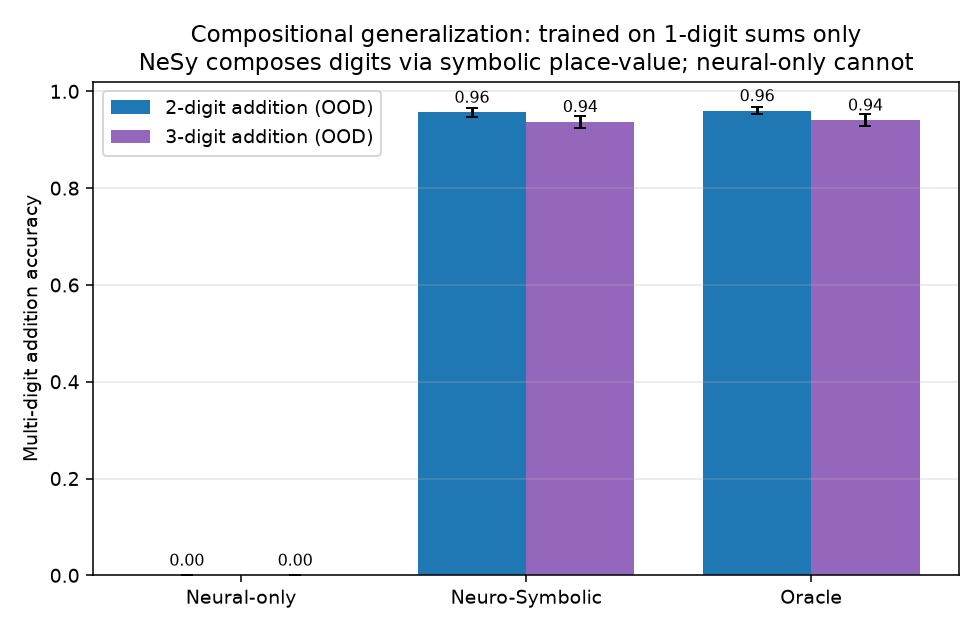
\includegraphics[width=0.7\linewidth]{figures/fig4_compositional_ood.png}
    \caption{Zero-shot compositional generalization. Trained only on single-digit sums, \nesy and the
    oracle solve $2$- and $3$-digit number addition at ${\sim}94$--$96\%$ by composing the digit
    classifier with a symbolic place-value sum. The \neural baseline scores $0\%$---it structurally
    cannot represent outputs in this range. Error bars are $95\%$ confidence intervals over $5$ seeds.}
    \label{fig:ood}
\end{figure}

\section{Discussion}
\label{sec:discussion}

\para{Integration is a real capability and data-efficiency win.} Wiring the symbolic operator into the
model factorizes the task into digit recognition, so \nesy learns from far fewer examples and matches a
fully supervised oracle (\secref{sec:e1}). Effect sizes are large at every size and overwhelming at
$1{,}000$ pairs ($d{=}56$). We provide what the literature usually only asserts: a head-to-head
learning-curve comparison with confidence intervals on identical splits.

\para{Whether high accuracy implies correct symbols is a property of the operator, not of NeSy.} This
is our central and most useful finding. Standard addition is shortcut-robust because its boundary sums
identify the digits; modular addition is shortcut-prone because its rotational symmetry does not. The
same network swings from $99.0\%$ grounding to $\approx0.1\%$ (among task-learning seeds) when we flip a
single operator, while the oracle---which sees digit labels---grounds at $99\%$ on \emph{both} operators,
the clean control (\secref{sec:e5}). The Hungarian-aligned metric is what makes the failure legible:
aligned grounding far above the raw value exposes a \emph{systematic} relabeling rather than noise, and
in the cleanest case the model lands on the exact algebraically predicted cyclic shift. The
methodological implication is direct: report grounding, and report it permutation-aligned; sum accuracy
alone is blind to this failure.

\para{The cure matches the disease.} When the problem is non-identifiability, supplying a tiny amount
of identifying information---$10$ labeled images, one per class---restores grounding to $97.7\%$ in every
seed and also removes the training instability (\secref{sec:e3}). Unsupervised regularizers, which add no
identifying information, mostly cannot. This reframes ``mitigation'' as ``supply the missing constraint''
and shows it is cheap when needed and unnecessary when not.

\para{Correct grounding is what compositional generalization stands on.} The single-digit-trained
\nesy model solves multi-digit addition at ${\sim}94$--$96\%$ because, and only because, its digit
classifier is correct; the neural baseline's structural $0\%$ is the foil (\secref{sec:e4}). We are
careful here: the near-perfect correlation between grounding and OOD accuracy spans models that all
ground well and has little spread, so we lean on the categorical contrast ($0\%$ vs.\ ${\sim}96\%$)
rather than over-reading the correlation.

\para{Surprises.} Two results were sharper than we expected. First, a single operator flip makes
correct grounding vanish so reliably---raw grounding $\approx0.1\%$ in every seed that learns the
task---and the model occasionally realizes the \emph{exact} $d\mapsto(d{+}5)$ permutation, together with
training instability ($4/5$ shortcut, $1/5$ outright collapse). Second, the neural baseline shows high
variance under modular addition at $30$k (four seeds at $0.96$--$0.97$, one stuck at $0.10$), hinting
that the modular task is genuinely harder to represent without the additive factorization.

\para{Error analysis.} \nesy's residual errors on standard addition fall on genuinely ambiguous digit
images, consistent with its ${\sim}99\%$ grounding---they are \emph{perceptual}. Its ``errors'' under
modular addition are not perceptual at all: they stem from a systematic global relabeling of the symbols
(\figref{fig:confusion}), which is precisely why high task accuracy survives them.

\subsection{Limitations}
\label{sec:limitations}
We are explicit about scope. (i) \emph{Single benchmark, single perceptual domain}: all results are on
MNIST digits; the mechanism (task symmetry $\Rightarrow$ (non)identifiability of symbols) should
transfer, but we did not test other modalities such as HWF or CLEVR. (ii) \emph{One symbolic
relaxation}: our \nesy model is a faithful compact re-implementation of the DeepProbLog/Scallop exact
marginalization, not a benchmark of those toolkits themselves. (iii) \emph{Low-spread correlation}: the
H4 correlation is suggestive only; we rely on the categorical contrast. (iv) \emph{GPU non-determinism
and modular instability}: atomic CUDA operations make runs not bit-identical even with fixed seeds, so
the specific permutation a modular run lands on---and whether a seed shortcuts or collapses---varies
across re-runs. The robust, re-run-invariant phenomenon is that under the modular operator correct
grounding never emerges (raw grounding $\approx0.1\%$ whenever the task is learned; the oracle always
grounds at $99\%$). Because modular \nesy is unstable, aggregate statistics over seeds, not single runs,
are the unit of inference, and \figref{fig:confusion} reads the saved grid rather than fresh retrains.
Standard-addition results reproduce across re-runs to within ${\pm}0.01$. (v) Modular addition is a
\emph{deliberately constructed} shortcut-inducer chosen for its exact, analyzable symmetry, not a
naturally occurring task.

\para{Broader implications.} For anyone deploying a NeSy system, the practical message is that task
accuracy is a necessary but not sufficient signal of understanding. Latent symbols can be confidently
and systematically wrong while every reported number looks healthy. Auditing grounding---and analyzing
the symbolic operator for symmetries that fail to identify the symbols---should be standard practice,
and where shortcuts are possible, a handful of labeled symbols is a cheap and reliable safeguard.

\section{Conclusion}
\label{sec:conclusion}

We asked when integrating a fixed symbolic operation with a shared neural classifier produces a system
that genuinely perceives and reasons, and answered it with a single controlled study on \mnistadd.
Integration (i) is a large, statistically significant capability and data-efficiency win that matches a
fully-supervised oracle and beats a neural baseline, most sharply with little data; (ii) recovers the
\emph{correct} latent symbols \emph{if and only if} the task's structure identifies them---when it does
not, as under modular addition, the system reaches high task accuracy through systematic reasoning
shortcuts that only a permutation-aware grounding metric can detect; (iii) is cheaply repaired with
about $10$ labeled symbols exactly when a shortcut exists; and (iv) when grounding is correct, unlocks
zero-shot compositional generalization to multi-digit addition (${\sim}95\%$) that the neural baseline
structurally cannot achieve ($0\%$).

\para{Key takeaway.} In neuro-symbolic systems, task accuracy is not enough: measure latent grounding
permutation-aligned, analyze the symbolic operator for symmetries that fail to identify the symbols, and
if shortcuts are possible add a handful of labeled symbols---the cheapest, most reliable fix, and one
that unsupervised regularization does not match.

\para{Future work.} We plan to (a) replicate the symmetry$\to$(non)identifiability mechanism on HWF and
a relational task such as CLUTRR; (b) probe richer shortcut-inducing operators (parity,
sum-mod-$m$ for various $m$) to map identifiability as a function of operator algebra; (c) compare our
compact marginalization against DeepProbLog and Scallop on the \emph{same} grounding metric; and (d)
study an active-learning loop that requests the minimum labeled symbols needed to break a detected
shortcut.


\bibliography{references}

\end{document}
